\chapter{Risks \& Safety}
\section{Risks}
The maximum sound pressure level that is allowed by SUVA is 140dB and the averaging level 8h/day has to be below 110dB.The averaging level $L_m$ is given as
\begin{equation}\label{5_Safety_eq:AveragingLevel}
    L_m = 10 \log_{10} \left (  \frac{1}{T} \int_0^T 10^{0.1 L_p(t)}dt\right ).
\end{equation}
This can be solved for the sound pressure level $L_p(t) = L_p$ if it is assumed to be constant over a certain time $\tau$.
\begin{equation}\label{5_Safety_eq:AveragingLevel_SPL}
    L_p = L_m - 10\log_{10}\left ( \frac{\tau}{8} \right )
\end{equation}
To calculate the sound pressure level at any given point the directivity of the used transducers has to be calculated. As explained in Section \todo{Section} the sound directivity can be calculated as
\begin{equation}\label{5_Safety_eq:Directivity}
    Q_D = \frac{2 p(0)^2}{\int_{0}^{\pi}p^2(\theta)\sin{\theta}d\theta}. 
\end{equation}
The sound pressure ratio emitted by the transducers according to the data sheet and according to own measurements, measurement setup explained in \todo, is displayed in \ref{5_Safety_fig:Directivity}.  
\begin{center}\label{5_Safety_fig:Directivity}
    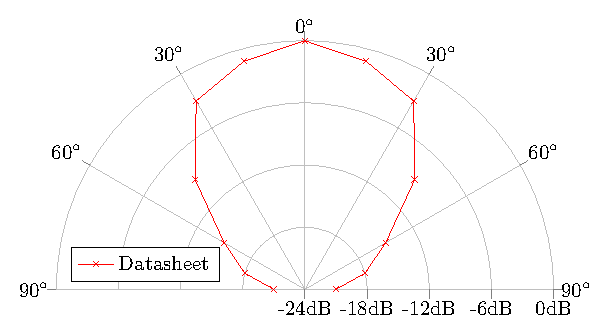
\includegraphics[width=0.9\textwidth]{images/5_Safety_Risks/Polar_PlotDirectivity.pdf}
\end{center}
With this information the directivity index turns out to be $Q_D = 22$ with which the maximum sound power level in relation to the distance of the listener can be calculated as
\begin{equation}
         L_{wmax} 
     = 
     \underbrace{L_{pmax}}_{140dB} - 10\left ( \underbrace{\log_{10}(Q_D)}_{1.35B} - \log_{10}(r^2) - \underbrace{\log_{10}(4\pi)}_{\approx 1.1B}  \right ) = 137.5 + 20\log_{10}(r).
\end{equation}
The maximum sound power allowed in relation to the distance is plottet in Figure \ref{5_Safety_fig:Max_power}.
\begin{center}
    \begin{minipage}{0.49\textwidth}\label{5_Safety_fig:Max_power_allowed}
    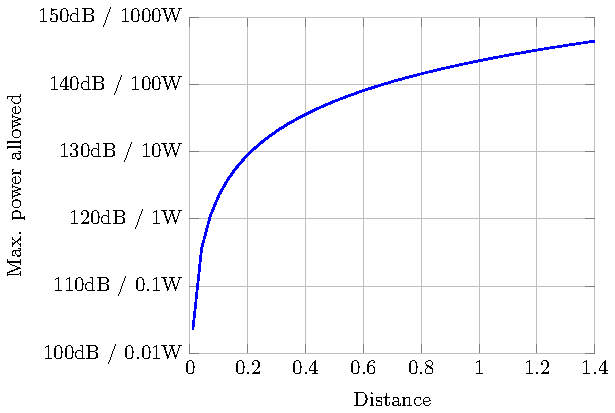
\includegraphics[width=\textwidth]{images/5_Safety_Risks/Max_Power_Allowed.pdf}
    \end{minipage}
    \begin{minipage}{0.49\textwidth}
    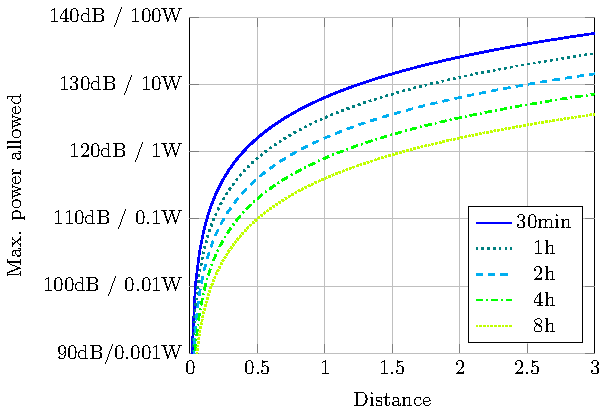
\includegraphics[width=\textwidth]{images/5_Safety_Risks/Max_Power_Allowed_Time.pdf}
    \end{minipage}
\end{center}
In Figure \todo it is shown what the maximum sound power allowed over different periods of time is calculated with Equation \ref{5_Safety_eq:AveragingLevel_SPL} where $L_m = 110dB$ as stipulate by SUVA.    
\section{Safety}
Through measuring the voltage over a resistor $R$ right in front of each line of transducer arrays the total current going into the transducers could be measured additionally the voltage was measured. Out of these measurements the total possible sound power which could be produced by the whole transducer array can be calculated
\begin{equation}
    L_{P,max} = M \cdot \frac{U_R}{R} U_{T}\eta_{T}.
\end{equation}
Where M is the number of channels, $U_R$ is the voltage over the resistor, $U_T$ is the voltage over the transducer and $\eta_{T}$ is the efficiency of the transducer. To guarantee maximal safety the efficiency $\eta_{T}$ is assumed to be one, which is a really high over estimation.
In this particular case the number of channels $M = 19$. For our loudspeaker the voltage are $U_R = 1.78 V$ and $U_T = 9.5 V $ and the resistor is $R = 22 \Omega$. This can be used to calculate the maximum sound power and with that the distance on which the device has to be muted to guarantee the safety of the ears of the listeners
\begin{equation}
     L_{P,max} = 19 \cdot \frac{1.78 V}{22 \Omega} 9.5 V = 14.36 W
\end{equation}
So to guarantee that a person could listen daily one hour to our loudspeaker on full volume without any harm the minimum distance was set to 2.5 meters. This distance is measured by a time of flight (ToF) sensor.    
\newpage